%File: feature.tex
%Author: Yuxin Wu <ppwwyyxx@gmail.com>

\subsection{Feature Detection and Matching}
\subsubsection{SIFT}
Lowe's SIFT algorithm\cite{sift} is implemented in \verb|feature/*.cc|.
The procedure of the algorithm and some results are briefly described as followed.
\begin{enumerate}
  \item \textbf{Scale Space} (\verb|feature/dog.cc|)

    A Scale Space consisting of $ S \times O$ grey images is built.
    The original image is resized in $ O$ different sizes (AKA. octaves), and each is then Gaussian-Blured
    by $ S$ different $ \sigma$.
    \begin{figure}[H]
      \centering
      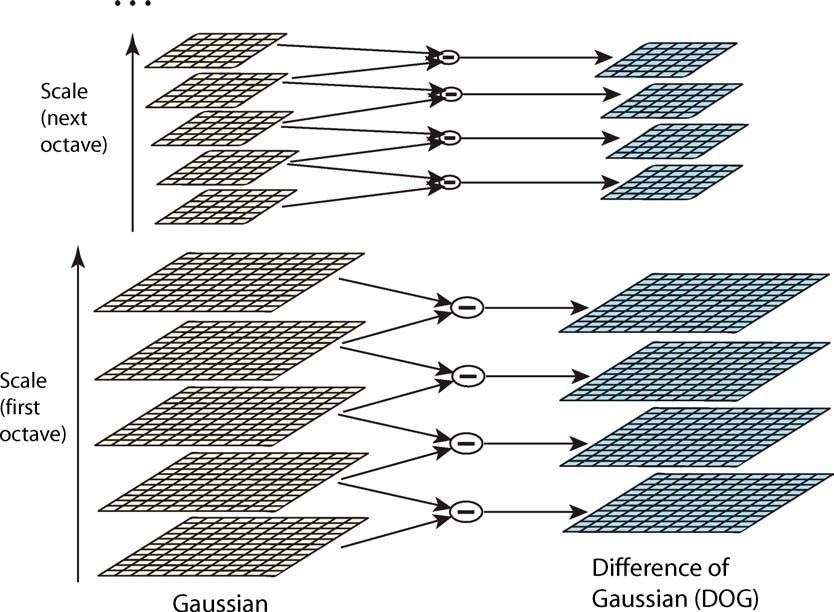
\includegraphics[scale=0.35]{res/dog.jpg}
      \caption{Scale Space and DOG Space \label{fig:dog}}
    \end{figure}

    Feature is detected on different resized version of the original
    image, to provide scale invariant feature.

    The gaussian blur here is implemented by applying two 1-D convolutions, rather than
    a 2-D convolution. This speeds up the computation significantly.

  \item \textbf{DOG Space}(\verb|feature/dog.cc|)

    In each octave, calculate the differences of every two adjacent blured images, to build a Difference-of-Gaussian Space.
    Therefore, DOG Space consists of $ (S - 1) \times O$ grey images.
    As shown in \figref{dog}.

  \item \textbf{Extrema Detection}(\verb|feature/extrema.cc|)

    In DOG Space, detect all the minimum and maximum
    by comparing a pixel with its 26 neighbors in \textbf{three directions}: $ x, y, \sigma$.
    See \figref{extrema} and \figref{extrema2}
    \begin{figure}[H]
      \begin{minipage}[b]{0.46\linewidth}
        \centering
        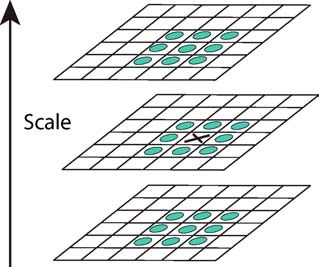
\includegraphics[scale=0.4]{res/extrema.png}
        \caption{Extrema Detection\label{fig:extrema}}
      \end{minipage}
      \hspace{1em}
      \begin{minipage}[b]{0.46\linewidth}
        \centering
        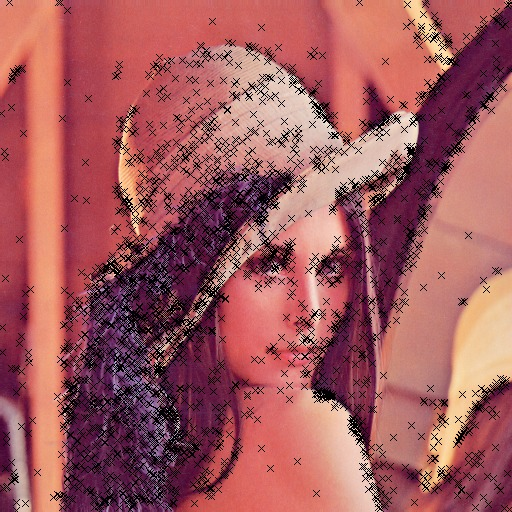
\includegraphics[scale=0.35]{res/extrema_lenna.png}
        \caption{Extrema Example\label{fig:extrema2}}
      \end{minipage}
    \end{figure}

  \item \textbf{Keypoint Localization}(\verb|feature/extrema.cc|)

    Use \textbf{parabolic interpolation} to look for the accurate location of the extrema.
    Then reject the points with \textbf{low contrast}(by thresholding pixel value)
    or \textbf{on the edge}(by thresholding principle curvature), to get more distinctive features.
    See \figref{feature1}, \figref{feature2}, \figref{feature3}.
    \begin{figure}[H]
      \begin{minipage}[b]{0.46\linewidth}
        \centering
        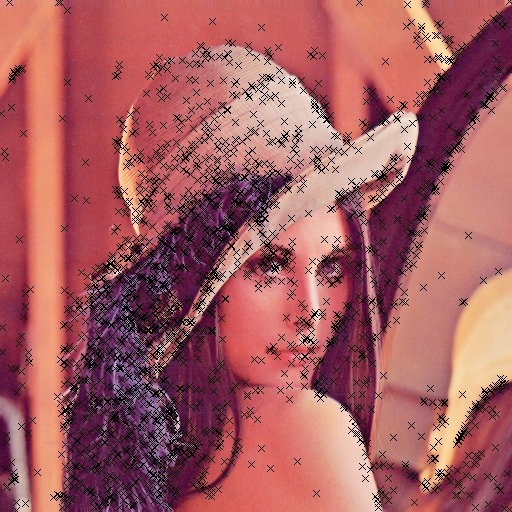
\includegraphics[scale=0.4]{res/feature_after_offset.png}
        \caption{After Localization \label{fig:feature1}}
      \end{minipage}
      \hspace{1em}
      \begin{minipage}[b]{0.46\linewidth}
        \centering
        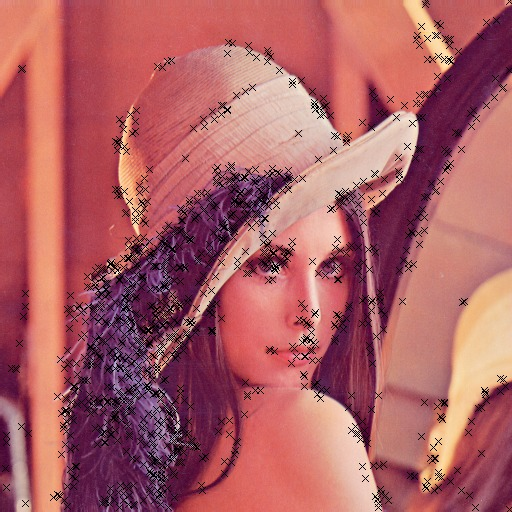
\includegraphics[scale=0.4]{res/feature_after_contrast.png}
        \caption{After Rejecting Low Contrast\label{fig:feature2}}
      \end{minipage}
    \end{figure}

  \item \textbf{Orientation Assignment}(\verb|feature/orientation.cc|)
    \label{sec:orientation_assign}

    First, we calculate \textbf{gradient and orientation} for every point in the Scale Space.
    For each keypoint detected by the previous procedure,
    the orientations of its nearby points will be collected and used to build an \textbf{orientation histogram},
    weighted by the magnitude of the gradient at each point, together with a gaussian kernel centered at the keypoint.
    The peak in the histogram is chosen to be the major orientation of the keypoint, as shown by the arrows in \figref{feature4}.

    \begin{figure}
      \begin{minipage}[b]{0.46\linewidth}
        \centering
        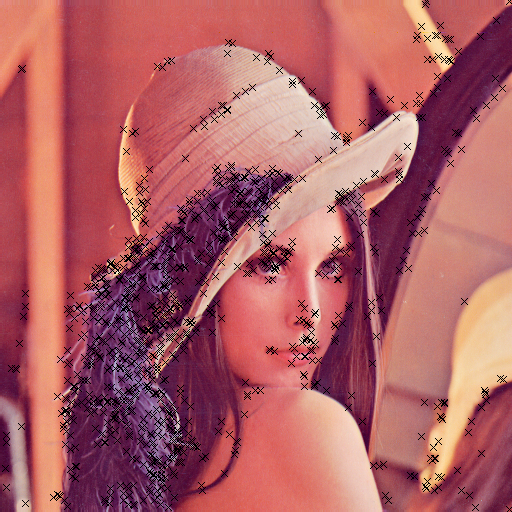
\includegraphics[scale=0.4]{res/feature_point.png}
        \caption{After Eliminating Edge Point\label{fig:feature3}}
      \end{minipage}
      \hspace{1em}
      \begin{minipage}[b]{0.46\linewidth}
        \centering
        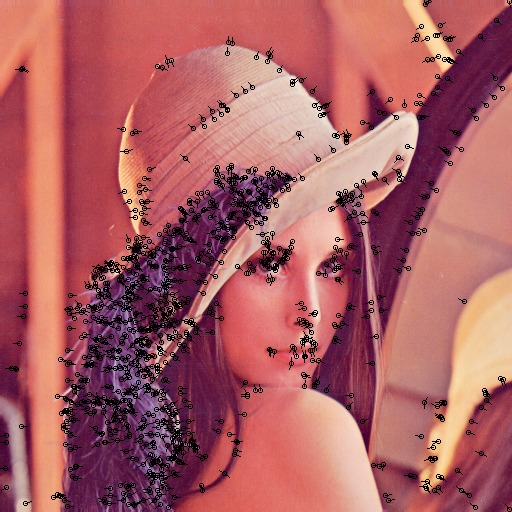
\includegraphics[scale=0.4]{res/feature_dir.png}
        \caption{After Assigning Orientation\label{fig:feature4}}
      \end{minipage}
    \end{figure}

  \item \textbf{Descriptor Representation}(\verb|feature/sift.cc|)

    D. Lowe suggested choosing 16 points around the keypoint, to build orientation histograms for each point, similar
    to the method in \secref{orientation_assign}.
    Each histogram uses 8 different possible values(bins). Therefore the final SIFT feature is a \textbf{128-dimensional}
    floating point vector.
    Since the major orientation of the keypoint is known, by using relative orientation to the keypoint,
    this feature is roatation-invariant.

  \item \textbf{Feature Matching}(\verb|feature/{feature,match}.cc|)

    \textbf{Euclidean distance} of the 128-dimensional descriptor is the criteria for feature matching between two images.
    A match is considered not convincing and therefore rejected,
    if the distances from it to its closest neighbor and second-closest neighbor are similar.
    A result is shown in \figref{match}.
    \begin{figure}[H]
      \centering
      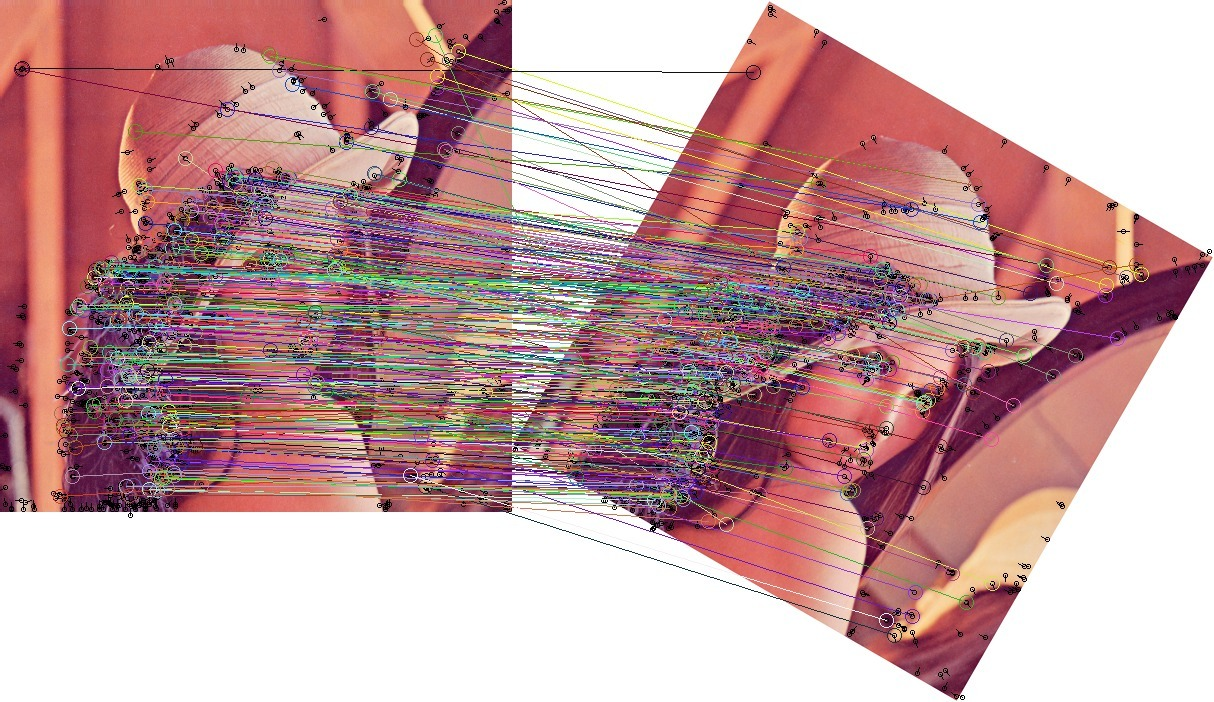
\includegraphics[width=\textwidth]{res/match.jpg}
      \caption{Matching Result\label{fig:match}}
    \end{figure}

    To calculate Euclidean distance of two arrays, I used Intel SSE3 intrinsics to speed up.
    KDTree could be used in the future to search for nearest neighbor.

\end{enumerate}

\subsubsection{BRIEF}
BRIEF is a simple and robust descriptor, details can be seen in \cite{brief}.

\begin{enumerate}
  \item \textbf{Keypoint}

    Keypoint localization in BRIEF feature can be done in different ways. I choosed to use the same routine as in SIFT feature.

  \item \textbf{Descriptor Representation}(\verb|feature/brief.cc|)

    BRIEF is computed by comparing 256 pairs of pixels around the keypoint. These pairs are pre-computed and fixed.
    Therefore the result would be a bit vector of 256 length.

  \item \textbf{Feature Matching}(\verb|feature/{match,feature}.cc|)

    \textbf{Hamming Distance} is used to compare two bit vectors.
    Similarly, a match is rejected if the distance to its nearest neighbor is similar to the distance to its second-nearest neighbor.
    The hamming distance is implemented with gcc \verb|__builtin_popcount()| function to speed up.

\end{enumerate}

